\subsection{Softwaresysteme}
Mit Software wird die Kommunikation zwischen externer Steuerungseinheit und Ballwurfmaschine, die Ortung des Korbes, sowie deren Konfiguration und die Steuerung der Motoren umgesetzt. In den folgenden Kapitel werden auf die einzelnen Komponenten eingegangen.

\subsubsection{Kommunikation zwischen externe Steuerungseinheit und Ballwurfmaschine}
Die Kommunikation erfolgt über Wireless LAN (WLAN). Das Raspberry PI, welches auf der Ballwurfmaschine installiert ist, stellt einen Access Point zur Verfügung mit welchem sich externe Steuerungseinheiten verbinden können. Die primäre externe Steuerungseinheit ist ein Notebook.\\
Auf dem PI werden Webservices angeboten, welche von dem Notebook aufgerufen werden können. Jede gängige Programmiersprache bietet Unterstützung für Webservices an. Dadurch schränkt man die Wahl der externen Steuerungseinheit nicht ein. Diese muss einzig den TCP/IP-Stack unterstützen. Die Webservices auf Seite des Raspberry PI werden mittels Python und mit Hilfe der Library web.py umgesetzt. Auf Seite der externen Steuerungseinheit gibt es eine Benutzeroberfläche, welche den Prozess anstossen kann (siehe UI-Skizze Bereich Ballwurf in Abschnitt \ref{ss-config-paramater-ortung-orb} ).

\subsubsection{Ortung des Korbes}
Der Ort des Korbes wird optisch bestimmt. Dazu wird zu Beginn des Prozesses ein Foto mittels der Raspberry PI Kamera geschossen. Dieses Bild wird anschliessend auf dem Raspberry PI mittels eines Algorithmus analysiert.\\
\\
\textbf{Algorithmus zur Ortung des Korbes}\\
Die grössten Herausforderungen stellen die unterschiedlichen Lichtverhältnisse dar. Der Algorithmus muss so robust sein, dass dieser damit umgehen kann. Generell sind mit Scheinwerfer von oben zu rechnen wobei der so Korb einen Schatten erhält. Auch Licht von der Seite durch die Fenster kann die Lichtverhältnisse beeinflussen.\\
\\
\textbf{Ablauf des Algorithmus}\\
\begin{figure}[h!]
	\centering
	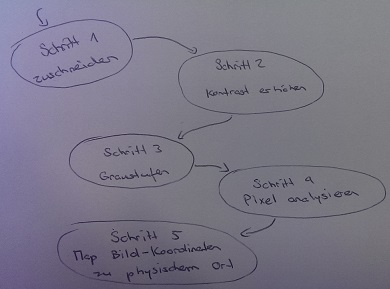
\includegraphics[scale=0.75]{../../fig/ablauf-algorithmus-orts-erkennung.jpg}
	\caption{Ablauf des Algorithmus}
\end{figure}

Auf der Abbildung sind die einzelnen Schritte zu erkennen, welche auf das Foto angewendet werden. Nachfolgend werden diese Schritte genauer erläutert:
\begin{itemize}
	\item Schritt 1 - Zuschneiden: Das Bild wird zugeschnitten. Irrelevante Informationen können so bereits eliminiert werden. Ausserdem hat es den positiven Effekt, dass das Bild physisch kleiner wird. Weitere Verarbeitungsschritte müssen so weniger Ressourcen aufwenden. 
	
	\item Schritt 2 - Kontrast verstärken: In diesem Schritt wird der Kontrast des Bildes erhöht. Das Histogramm verbreitert sich und helle Punkte werden noch heller und dunkle Punkte noch dunkler. Sprich der schwarze Korb wird noch intensiver erkennbar. 
	
	\item Schritt 3 - Graustufen setzen: Das Bild wird in Graustufen konvertiert. Dies hat zur Folge, dass jedes Pixel im Bild jeweils einen gleich hohen Anteil an rot, blau und grün Werten hält. Tiefe Werte bedeuten, dass der Punkt dunkel ist, hohe Werte entsprechend hell. (RGB(0,0,0) = schwarz, RGB(255,255,255) = weiss).
	
	\item Schritt 4 - Pixel analysieren: Es wird eine definierte Linie auf dem Bild analysiert. Nun ist auf dieser Linie ein längerer Bereich recht dunkel im Verhältnis zu den anderen Bereichen. Da kann nun angenommen werden, dass dort der Korb ist. Um das Problem mit dem Schatten zu umgehen, wird eine Linie analysiert welche möglichst weit oben im Bild ist, denn die Schatten könnten den Korb unten künstlich verbreitern.
	
	\item Schritt 5 - Umwandlung Bild-Koordinaten zu physischem Ort: Sobald der Punkt des Korbes auf dem Bild bekannt ist, kann der physische Ort bestimmt werden. Da die Kamera immer am gleichen Ort ist und der Zuschnitt des Bildes gleich erfolgt, kann eine Mapping-Tabelle dafür verwendet werden. In dieser Tabelle findet man die Zuweisung des Bild-Punktes zu dem physischen Ort. Als Output erzeugt der Algorithmus den Winkel zwischen Korb und Kamera.
\end{itemize} 
Die Raspberry PI Kamera kann bereits einige Schritte gleich selbst durchführen. Dazu zählen Schritt 1, 2 und 3 (siehe Abschnitt \ref{ss-schnittstelle-raspistill}). Das heisst der Algorithmus muss sich selbst nicht um diese Transformationen kümmern, muss also nur die Parameter an die Kamera weiterreichen.\\
\\
Die Schritte 4 und 5 müssen jedoch auf dem Raspberry PI implementiert werden.

\begin{lstlisting}[language=Python]
from PIL import Image
bild = Image.open('korb.jpg')
pixelarray = bild.load()
print (pixelarray[10,10])
pixelarray[10,10] = (0,0,0)
print (pixelarray[10,10])
\end{lstlisting}

Auf der Abbildung ist zu erkennen wie man ein Pixel auslesen kann.\\
\\
Alle Parameter für die einzelnen Schritte des Algorithmus müssen konfigurierbar sein. Beim Einrichten der Ballwurfmaschine dürfen fünf Minuten verwendet werden. In dieser Zeit sollen diese Parameter der Umgebung angepasst werden können (siehe Abschnitt \ref{ss-config-paramater-ortung-orb}).\\
\\
\textbf{Implementierung}\\
Die Implementation erfolgt in Python auf dem Raspberry PI. Python ist bewährt und bietet viele Bibliotheken. Verwendet wird die Version 2, denn Version 3 ist seit langem released, konnte sich aber noch nicht endgültig durchsetzen. Viele Libraries wurden noch immer nicht portiert. Zur Verwendung kommt die Bibliothek Pillow mit welchem man simple Bildoperationen durchführen kann. Zum anderen wird die Picamera Library verwendet um die Kamera anzusteuern.

\subsubsection{Ballwufmaschine-UI}
\label{ss-config-paramater-ortung-orb}
Damit die Parameter angepasst werden können, wird eine Software auf Seite der externen Steuerungseinheit implementiert. Diese Komponente besitzt ein UI, welches in Java programmiert wird.

\begin{figure}[h!]
	\centering
	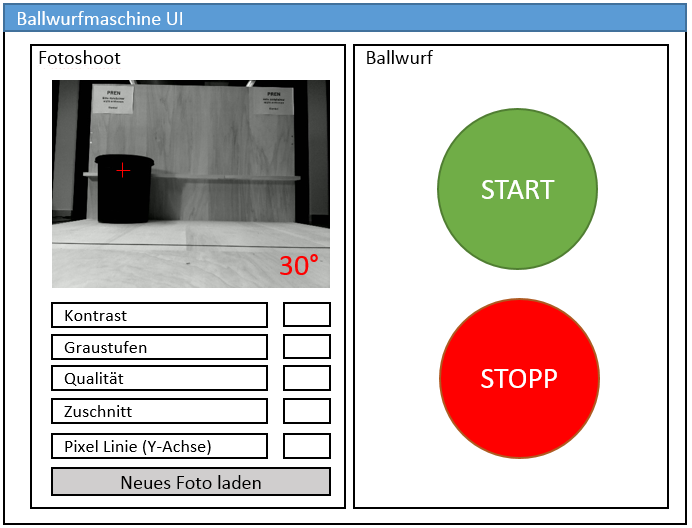
\includegraphics[scale=0.75]{../../fig/fotoshoot-configurator.png}
	\caption{Ballwurfmaschine-UI Skizze}
\end{figure}

Das UI der Ballwurfmaschine lässt im Bereich Fotoshoot alle relevanten Werte konfigurieren. Es erhält jeweils das aktuelle Foto, welches in diesem Prozess mit Informationen angereichert wird. Der Algorithmus markiert den Korb mit einem Fadenkreuz und schreibt den Winkel unten rechts aufs Bild.

\subsubsection{Steuerung der Motoren}
TODO Ervin